\input format.tex

\usepackage{graphicx}
\graphicspath{{cores/}}

\begin{document}

\vspace*{8mm}
%% 各章节
\setlength{\arrayrulewidth}{1pt}
\fontsize{9.3pt}{11pt}\selectfont
\color{gray2}
\begin{center}
{\noindent\bf\sanhao 一、肠道菌群多样性结果解析}
\end{center}

\vspace*{6mm}
{\noindent\bf\wuhao 肠道菌群多样性}

\begin{LRaside}[.8]{检测说明}
\noindent
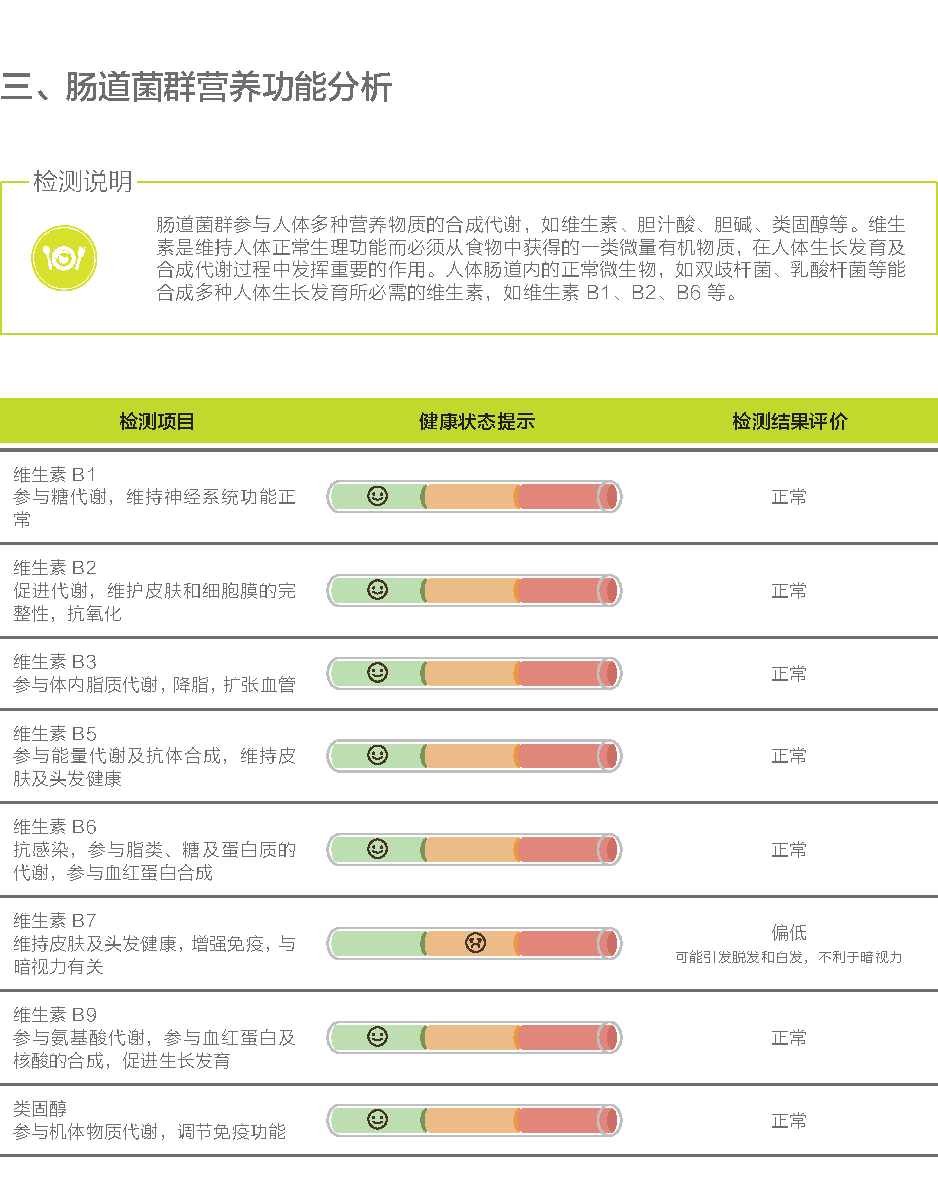
\includegraphics[width=\linewidth]{yingyanggongneng.pdf}
\asidebreak %
人体肠道内存在上万亿个细菌,不同菌群共同组成了复杂的肠道微生态系统。国际最新权威研究发现,肠道微生态与肥胖关系密切,因此,通过检测发现导致肠道微生态失衡的已有或潜在因素,有效减重或预防肥胖的发生。
\end{LRaside}
\smallskip
{\noindent\bf\wuhao 检测结果}
\vspace*{-5mm}
\begin{center}
\setlength{\unitlength}{1cm}
\begin{picture}(15,9)(0,-2)
%\put(0,5.7){\bfseries 您的肠道菌群多样性为:2.80(参考范围:1.50-4.41)}
%\put(0,5.7){\bfseries 您的肠道菌群多样性为:2.80}
%\put(0,6.5){\bfseries 检测结果}
\put(0.7,6){\bfseries 多样性(参考范围:1.50-4.41)}
\put(0.7,0){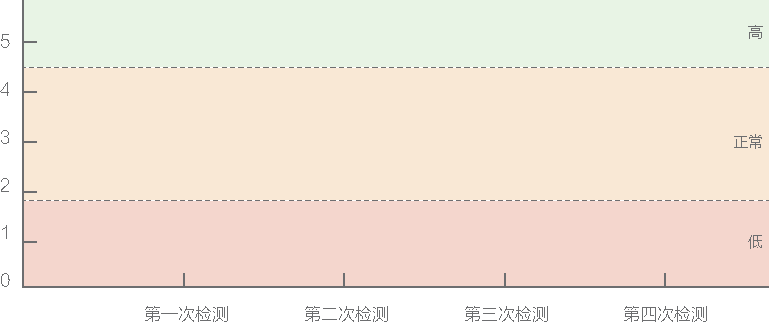
\includegraphics[width=.85\linewidth]{diversity_region.pdf}}
\put(3.79,2.8533){\tikz\draw[topcolor,fill=topcolor](0,0) circle[radius=3.5pt];}
\put(3.19,3.2533){\bf\bahao 本次检测值2.80}
%\put(2.8533,.5){
\includegraphics[width=1.29cm]{location.pdf}}
%\put(10.7,.5){
\includegraphics[width=1.29cm]{diversity20.pdf}}
%\put(10.7,4.5){\parbox{2cm}{\color{topcolor}\bfseries 您的数值高\\于21{\%}\\的参考人群。}}
%\put(0,-.5){肠道菌群多样性分布图(紫色虚线标示了您的位置,红色虚线之间是参考区域)}
\end{picture}

\end{center}

\vspace{-1.2cm}
\begin{LRaside}[.8]{结果分析}
\noindent
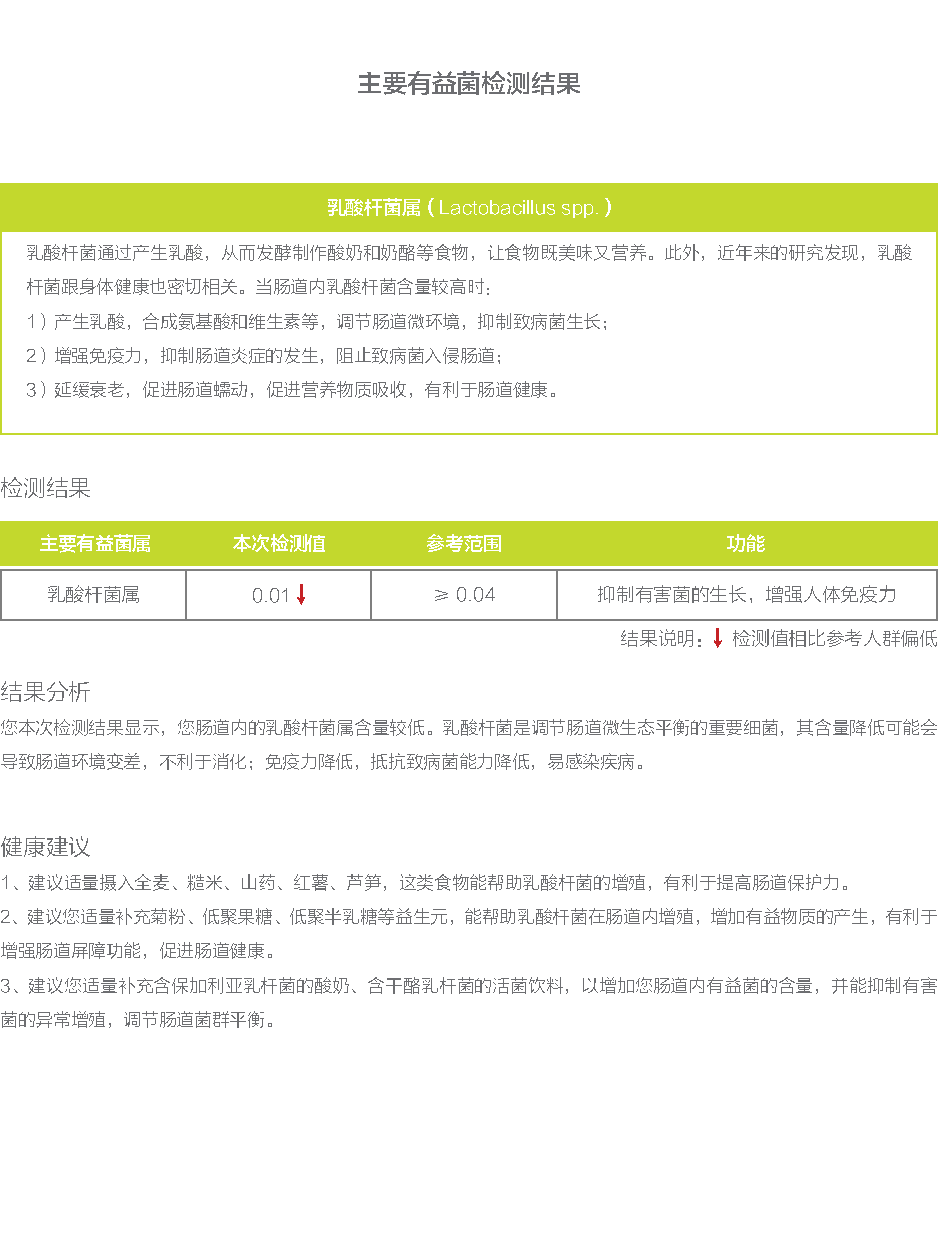
\includegraphics[width=\linewidth]{result.pdf}
\asidebreak %
您的肠道菌群多样性正常,说明您的肠道菌群组成较为丰富,菌群失调风险较低。您的肠道菌群不易受到外界因素的干扰,但仍需避免不良作息、刺激性食物、药物滥用等的影响,这样有助于保持较好的肠道菌群多样性,增强机体新陈代谢和免疫能力。
\end{LRaside}

\end{document}

